\documentclass{article}
\usepackage[utf8]{inputenc}
\usepackage{tikz}
\usetikzlibrary{calc}
\begin{document}
\section{ Question  18 MUX diagram }
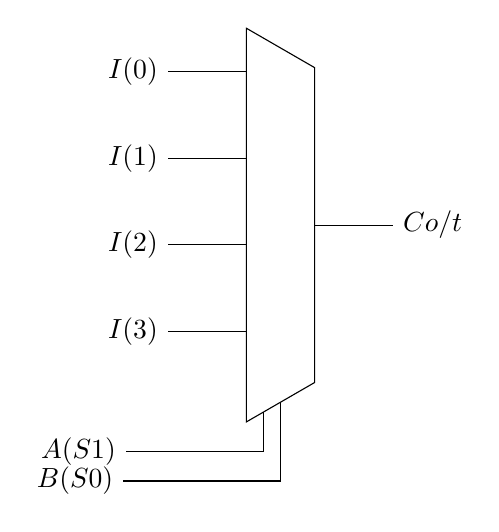
\begin{tikzpicture}
\draw (0,0)coordinate (O)--++(30:1)coordinate (P)--++(90:4)coordinate (Q)--++(150:1)coordinate (R)--cycle;
\draw($(P)!0.5!(Q)$)--++(0:1)node[right]{$Co/t$};
\draw($(O)!0.5!(P)$)--++(-90:1)--++(180:2)node[left]{$B(S0)$};
\draw($(O)!0.25!(P)$)--++(-90:0.5)--++(180:1.75)node[left]{$A(S1)$};
\foreach\y/\t in {0.1/(0),0.3/(1),0.5/(2),0.7/(3)} {
\draw ($(R)!\y*1.1!(O)$)--++(180:1)node[left]{$I\t$};}
\end{tikzpicture} 


    
\end{document}
